\documentclass{beamer}
%\usepackage{beamerthemedefault}
\usepackage[utf8]{inputenc}
\usepackage[portuges]{babel}
\usepackage{subfigure}  
\usepackage{multirow}
\usepackage{listings}
\usepackage{moreverb}
% Vary the color applet  (try out your own if you like)
%\colorlet{structure}{red!65!black}

%\beamertemplateshadingbackground{white!100}{white}

% \usetheme{AnnArbor}
% \usetheme{Ilmenau}
% \usetheme{Antibes}
% \usetheme{JuanLesPins}
% \usetheme{Bergen}
% \usetheme{Luebeck}
% \usetheme{Berkeley}
% \usetheme{Madrid}
% \usetheme{Berlin}
% \usetheme{Malmoe}
% \usetheme{Boadilla}
% \usetheme{Marburg}
% \usetheme{boxes}
% \usetheme{Montpellier}
% \usetheme{CambridgeUS}
% \usetheme{PaloAlto}
 \usetheme{Copenhagen}
% \usetheme{Pittsburgh}
% \usetheme{Darmstadt}
% \usetheme{Rochester}
% \usetheme{default}
% \usetheme{Singapore}
% \usetheme{Dresden}
% \usetheme{Szeged}
% \usetheme{Frankfurt}
% \usetheme{Warsaw}
% \usetheme{Goettingen}
% \usetheme{Hannover}

%    \usecolortheme{albatross}% - modre ramecky, jinak modre pozadi
%    \usecolortheme{beetle}% - namodrale ramecky, sede pozadi
%    \usecolortheme{beaver}% - namodrale ramecky, sede pozadi - branco + cinza
%    \usecolortheme{crane}% - zlute ramecky, bile pozadi - amarelo
%    \usecolortheme{sidebartab}% - namodrale ramecky, sede pozadi
%    \usecolortheme{wolverine}% - namodrale ramecky, sede pozadi
%    \usecolortheme{default}%
%    \usecolortheme{dolphin}% - bile a sedomodre ramecky, podobne default, svetlejsi
%    \usecolortheme{dove}% - bile ramecky, skoro cernobile
%    \usecolortheme{fly}% - sede pozadi i ramecky, nadpisy bile
%    \usecolortheme{lily}% - skoro stejne jako default, jen bile ramecky nadpisu
%    \usecolortheme{orchid}% - stejne jako default?
%    \usecolortheme{rose}% - stejne jako default?
%    \usecolortheme{seagull}% - podobne dolphin, sede ramecky, bile pozadi
%    \usecolortheme{seahorse}% - podobne dolphin, sede ramecky, bile pozadi
%    \usecolortheme{whale}% - stejne jako default?

\setbeamertemplate{items}[ball]
\setbeamercolor{subitem projected}{bg=red} 
\setbeamercolor{item}{bg=white}
\setbeamercolor{item}{fg=red} 
% 
%
\lstset{
 numbers=left, 	% where to put the line-numbers
%stepnumber=5,
firstnumber=1,
numberstyle=\tiny,
extendedchars=true,
breaklines=true,
frame=tb,
basicstyle=\footnotesize, %the size of the fonts that are used for the code
stringstyle=\ttfamily
captionpos=b,                   % sets the caption-position to bottom
tabsize=2,
showstringspaces=false
}
\title{Scala: Primeiros passos com o paradigma funcional}
\setbeamercolor{item}{bg=white}
 \setbeamercolor{item}{fg=red} 
%==================================================
%=============== Dados da Apresentação ============

%\date{\today}
\author[Diego, Ronualdo]{
	Diego Saraiva \\
	Ronualdo Maciel
}
 
% \subject{primeiro slide}
\usepackage{amsmath}
\begin{document}
\rmfamily

%\Large
\frame{
	\titlepage
	\begin{center}
		\date{\today}
	\end{center}
}

\section{Quem somos}

\begin{frame}
	\begin{block}{Diego Saraiva - diegosaraiva@gmail.com}
		Mestre em sistemas distribuídos pela UFRN tendo atuado como desenvolver e
		pesquisador em diversos projetos.
	\end{block}
	
	\begin{block}{Ronualdo Maciel - raxmac@gmail.com}
		Desenvolvedor de software desde 2005 atuando principalmente no desenvolvimento
		de aplicações java (Web/Desktop.)
	\end{block}
\end{frame}

 %==================================================slide
% % cria o sumário
 \begin{frame}
  \frametitle{Sumário}
  \tableofcontents [pausesections]
 \end{frame}
%-------------------------------------------------------
%==================================================slide\documentclass{beamer}

\section{Introdução}
\begin{frame}{Introdução}
	\begin{block}{Exigências do mercado atual}
		\begin{itemize}
			\item Utilização efetiva de máquinas multi-core por programas concorrentes. 
			\item Criação de aplicações distribuídas voltadas para a Web ou para a Internet.
		\end{itemize}
	\end{block}
\end{frame}

\begin{frame}{Introdução}
    \begin{block}{Linguagens}
        \begin{center}
	        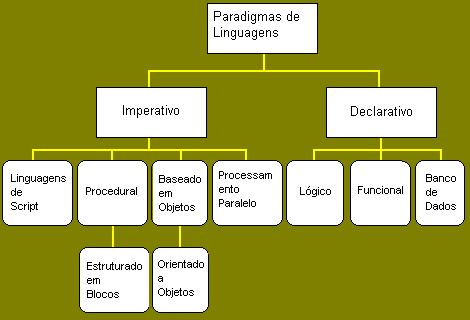
\includegraphics[scale=0.4]{paradigmas-imagem.png} 
        \end{center}
    \end{block}
\end{frame}

\begin{frame}{Introdução}
	\begin{block}{Programação orientada a objetos}
		\begin{itemize}
			\item Estilo imperativo 
			\item Tenta simular o mundo real
			\item A computação é realizada em termos de estados e expressões que podem
			mudar o estado do programa.
		\end{itemize}
	\end{block}
	\begin{center}
		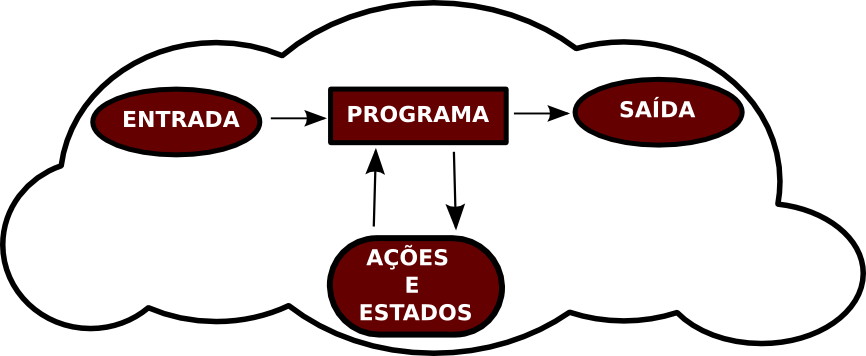
\includegraphics[scale=0.3]{progImp.png}
	\end{center}
\end{frame}

\begin{frame}{Introdução}
	\begin{block}{A Programação Funcional}
		\begin{itemize}
			\item Estilo de programação baseado no uso de funções
			\item Funções são entidades de 1ª classe 
			\item Toda a programação é baseada na avaliação de expressões para gerar valores. 
			\item Cada valor tem um tipo associado.
			\item Funções podem ser nomeadas ou anônimas (lambda)
		\end{itemize}
	\end{block}
\end{frame}

\subsection{Apresentando Scala}
% contextualizar a linguagem
\begin{frame}{Introdução}
	\begin{block}{Scala}
        \begin{itemize}
            \item O nome Scala significa ``linguagem escalável"
            \item Projetada para integrar linguagem orientada a objetos e programação funcional
            \item Executa na JVM
        \end{itemize}
	\end{block}
\end{frame}

\begin{frame}{Scala}
    \begin{block}{Histórico}
        \begin{itemize}
            \item O design começou em 2001 na École Polytechnique Fédérale de Lausanne por Matin Odersky
            \item Primeiro release na plataforma Java: no fim de 2003 e início de 2004 
            \item Versão para plataforma .NET liberada em Junho de 2004
        \end{itemize}
    \end{block}
\end{frame}
%propraganda, doutrinar o povo, enfim igual a java
\subsection{Por que utilizar Scala?}

\begin{frame}{Scala}
    \begin{block}{Por quê utilizar Scala?}
        \begin{itemize}
            \item Linguagem híbrida: simplicidade de funcional + poder de objetos
            \item Fortemente tipada
            \item Linguagem Concisa
            \item Multiplataforma: JVM e .NET 
        \end{itemize}
    \end{block}
\end{frame} 

%motivação tecnica
\subsection{Uma Linguagem Escalável}


\section{Paradigma Funcional}
\begin{frame}{Introdução a programação funcional}
	\begin{block}{Entidades de primeira-classe}
	\begin{itemize}
		\item Entidades que podem ser passadas como parâmetro
		\item Podem ser retornadas como resultado
		\item Podem ser armazenadas em estruturas de dados
	\end{itemize}
	\end{block}
\end{frame}
\begin{frame}{A Programação Funcional}
	\begin{block}{Modelo computacional}
		\begin{itemize}
			\item Função de x em y : Mapeamento de valores de entrada em valores de saída
			\item Ausência de estado e comandos (atribuição + controle)
		\end{itemize}		
	\end{block}
	\begin{center}
		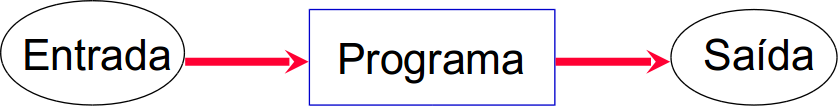
\includegraphics[scale=0.3]{modelo_funcional.png}
	\end{center}
\end{frame}
\begin{frame}{Paradigma Funcional}
	\begin{block}{Mudando o foco}
		\begin{itemize}
			\item sem laços?
			\item sem efeitos colaterais?
			\item sem mudar o valor de variáveis?
		\end{itemize}
	\end{block}
	\begin{block}{Aplicações}
		\begin{itemize}
			\item Verificação de programas: checagem de corretude 
				\begin{itemize}
					\item Princípio da invariância. 
				\end{itemize}
			\item Otimização de programas para computação paralela
		\end{itemize}
	\end{block}
\end{frame}
\begin{frame}{Paradigma Funcional}
	\begin{block}{Linguagem Funcional}
		\begin{itemize}
			\item O corpo de uma função é uma expressão
			\item A aplicação da função a um argumento retorna um valor (expressão)
			\item Um programa é uma expressão
		\end{itemize}		
	\end{block}
	\begin{block}{O contexto}
		\begin{itemize}
			\item Mapeamento de identificadores (nomes de função) em definições de função
			\item Mapeamento de identificadores em valores  
		\end{itemize}
	\end{block}
\end{frame} 

\section{Sintaxe}

\begin{frame}{Sintaxe}
	\begin{block}{Variáveis}
		\lstinputlisting{sintaxe_scala/codigo/variaveis.scala}
	\end{block}
\end{frame}

\begin{frame}{Sintaxe}
	\begin{block}{Definição de métodos}
		\lstinputlisting{sintaxe_scala/codigo/metodos.scala} 
	\end{block}
\end{frame}

\begin{frame}{Sintaxe}
	\begin{block}{Chamadas a métodos}
		\lstinputlisting{sintaxe_scala/codigo/chamadas_metodos.scala} 
	\end{block}
\end{frame}

\begin{frame}{Sintaxe}
	\begin{block}{Classes - Scala}
		\lstinputlisting{sintaxe_scala/codigo/classes.scala}
	\end{block}
	
	\begin{block}{Classes - Java}
		 \lstinputlisting{sintaxe_scala/codigo/classes.java}
	\end{block}
\end{frame}

\begin{frame}{Sintaxe}
	\begin{block}{Classes - Scala}
		\lstinputlisting{sintaxe_scala/codigo/classes_get.scala} 
	\end{block}
	
	\begin{block}{Classes - Java}
		 \lstinputlisting{sintaxe_scala/codigo/classes_get.java}
	\end{block}
\end{frame}

\begin{frame}{Sintaxe}
	\begin{block}{If}
		 \lstinputlisting{sintaxe_scala/codigo/if.scala}
	\end{block}
\end{frame}

\begin{frame}{Sintaxe}
	\begin{block}{For}
		 \lstinputlisting{sintaxe_scala/codigo/for.scala}
	\end{block}
\end{frame}

\begin{frame}{Sintaxe}
	\begin{block}{While}
		 \lstinputlisting{sintaxe_scala/codigo/while.scala}
	\end{block}
\end{frame}

\begin{frame}{Sintaxe}
	\begin{block}{Try}
		 \lstinputlisting{sintaxe_scala/codigo/try.scala}
	\end{block}
\end{frame}

\begin{frame}{Principais conceitos}
	\begin{block}{Funções como entidades de primeira ordem} 
		\begin{itemize}
			\item As funções podem ser criadas em qualquer lugar do programa
			\item As funções podem armazenadas em estruturas de dados
			\item As funções podem ser passadas como argumento para outras funções
			\item As funções podem retornar outras funções como resultados
		\end{itemize}
	\end{block}
	
	\begin{center}
		\lstinputlisting{conceitos/exemplos/funcoes.scala}
	\end{center}
\end{frame}

\begin{frame}{Principais conceitos}
	\begin{block}{Funções de alta-ordem}
		\begin{itemize}
			\item Recebem uma ou mais funções como entrada
			\item Retornam uma função como saída
			\begin{itemize}
				\item Exemplo: map
			\end{itemize}
		\end{itemize}
	\end{block}
\end{frame}

%Uma closure ocorre normalmente quando uma função é declarada dentro do corpo de outra,
%e a função interior referencia variáveis locais da função exterior. Em tempo de execução, 
% quando a função exterior é executada, então uma closure é formada, que consiste do código 
%da função interior e referências para quaisquer variáveis no escopo da função exterior que a closure necessita.
\begin{frame}{Principais conceitos}
	\begin{block}{Closures}
		\begin{itemize}
			\item Um closure é uma função que referencia variáveis livres no contexto léxico. 
			\item Função anônima definida on-the-fly dentro de uma função ou expressão
			\item Uma closure pode ser definida pelo compilador como resultado de outra função
			\item Closure é diferente de uma função anônima
		\end{itemize}
	\end{block}
	
	\begin{center}
		\lstinputlisting{conceitos/exemplos/closures.scala}
	\end{center}
\end{frame}


\begin{frame}{Principais conceitos}
	\begin{block}{Currying}
		%technique of transforming a function that takes multiple arguments 
		% (or an n-tuple of arguments) in such a way that it can be called as 
		% a chain of functions each with a single argument.
% 		Uma função "curried" transforma uma função que recebe múltiplos parâmetros em uma função que 
		%pode ser chamada como uma cadeia de funções que recebem somente um parâmetro
		%cada vez.
		Currying é o processo de transformar uma função que recebe múltiplos
		argumentos em uma função que recebe um único argumento e retorna outra função.
	\end{block}
	%\begin{block}{Visão informal}
	%	Uma função "curried" quando ela possui mais de uma lista de parâmetros, sendo
	%	assim, a mesma função
	%	é invocada em cadeia para cada lista de parâmetro.
	%\end{block}
	
	\begin{center}
		\lstinputlisting{conceitos/exemplos/curry.scala}
	\end{center}
\end{frame}
 
\begin{frame}{Principais conceitos}
	\begin{block}{Pattern Matching}
	Pattern matching é uma forma de associar nomes a coisas e possivelmente quebrar as expressões
	em sub-expressões ao mesmo tempo em que associa cada sub-expressão a cosias.
		\begin{itemize}
			\item Reconhecer valores
			\item Associar variáveis para reconhecer valores
			\item ``Quebrar" valores em partes
		\end{itemize}
	\end{block}
	
	\begin{center}
		\lstinputlisting{conceitos/exemplos/match.scala}
	\end{center}
\end{frame}

\section{Exemplos}

\begin{frame}{Exemplos}
	\begin{block}{ }
		\textbf{Some code\ldots}
	\end{block}
\end{frame}

\section{Mais Informações}

\begin{frame}{Livros}
	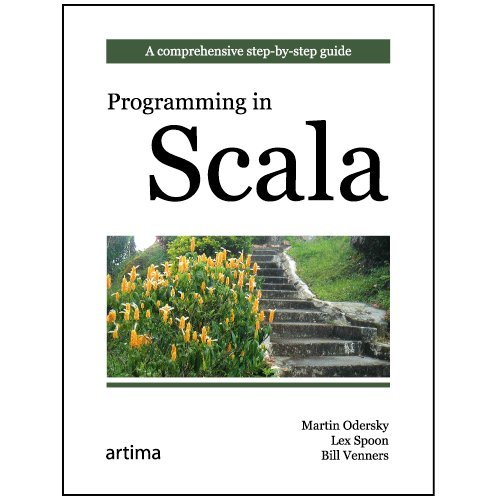
\includegraphics[scale=0.3]{conclusao/progInScala.jpg}
	
\includegraphics[scale=0.4]{conclusao/beginning-scala.jpg}
\end{frame}

\begin{frame}{Sites}
	\begin{block}{ }
		\begin{itemize}
			\item \textbf{Site oficial -} http://www.scala-lang.org/
			\item \textbf{Blog Scala-BR -} http://scala-br.org/
			\item \textbf{Grupo Scala-BR -} http://groups.google.com/group/scala-br 
		\end{itemize}
	\end{block}
\end{frame}

\section{Perguntas}

\begin{frame}{Fim}
	\begin{block}{ }
		\begin{center}
			\textbf{Perguntas ???}
		\end{center}
	\end{block}
\end{frame}

\end{document}
